\chapter{Hydraulics}
This compendium on hydraulics is based on Jim Pytel excellent course called ``Hydraulics Training'' on YouTube. I highly recommend viewing it, its also more correct than what is written in this compendium since Mr. Pytel is much more knowledgeable about Hydraulics than me. Additional, Yuken Kogyo Co.,LTD has an great book on hydraulics~\cite{yuken2006basic}.


\section{Introduction and Fluid Properties}
Hydraulics systems transfer power by fluid within a close system. The advantage over pneumatic systems, which uses air, is that most fluids are incompressible, resulting in the ability of hydraulic actuators, e.g., hydraulic cylinder, to hold its position even under high loads. 

% Compressability
A substance's resistance to uniform compression is measured in terms of Bulk modulus ($B$), $B = \Delta{P}/(\Delta{V}/V)$, where $P$ is pressure and $V$ is volume. For water the bulk modulus is 2190 MPa~\cite{brennen_fluid_dynamics} in 20 C and in typical heavy machinery application the pressure is between 20–35 MPa, meaning that the volume will only decrease about 9-15.9 mL for each liter of water. Water is typically not used in hydronic systems, instead mineral-based hydraulic oil that are derived from crude oil or synthetic-based hydraulic oil, which have a slightly lower bulk module. But even for high pressure systems 50 MPa under 20 C the bulk modulus is 1880 MPa~\cite{gholizadeh_fluid_bulk_modulus}, resulting a volume decrease of....  Temperature has a greater effect on volume, however, both need to be taken into account.

% Lubricant
Mineral-based and synthetic-based hydronic oil has additional properties over water, it acts as a lubricant. It also provides a seal for hydraulic cylinders, unlike water that could leak between chambers?

% Viscosity
Another properties...


% Oil and no other fluid since its a lubricant.
% What is it good for, much stronger and can keep its position. Fluids are not compressable.
% Very basic about the varius components


\section{Pascals Law with Examples for Hydraulic Systems}
\subsection{Pascals Law}
A pressurized static fluid in a closed vessel exerts pressure equally in all direction throughout the fluid and works octagonal on a plane. Pressure ($P$ [$Pa$ or $psi$]) can be expressed  as a fraction of the force ($F$ [$Nm$ or $lbf$]) per unit area ($A$ [$m^2$ or $in^2$]). 
\begin{equation*}
  P = \frac{F}{A}
\end{equation*}

\subsection{Force Multiplier}
A small weight providing small force can lift a large weight requiring large force.
\begin{figure}[H]
\centering
\begin{tikzpicture}
  \coordinate (BL) at (0,0);  % Bottom left
  \coordinate (BR) at (6,0);  % Bottom right
  \coordinate (TL) at (0,4);  % Top left 
  \coordinate (TR) at (6,4);  % Top right

  \coordinate (BCL) at (1,0.5);  % Bottom center left
  \coordinate (BCR) at (2.5,0.5);  % Bottom center right
  \coordinate (TCL) at (1,4);  % Top center left 
  \coordinate (TCR) at (2.5,4);  % Top center right

  \draw (TL) -- (BL) -- (BR) -- (TR);
  \draw (TCL) -- (BCL) -- (BCR) -- (TCR);

  \draw ([shift={(0.1,0)}]TL) rectangle ([shift={(-0.1,-0.4)}]TCL);
  \draw ([shift={(0.1,0)}]TCR) rectangle ([shift={(-0.1,-0.4)}]TR);

  \fill ([shift={(0.25,0)}]TL) rectangle ([shift={(-0.25,0.8)}]TCL)node[above=2mm] {$\SI{40}{\kilo\newton}$};
  \fill ([shift={(0.40,0)}]TCR) rectangle ([shift={(-0.40,0.8)}]TR) node[above=2mm] {$\SI{1000}{\kilo\newton}$};

  \draw[dashed] ([shift={(0.1,-1)}]TL) rectangle ([shift={(-0.1,-1.4)}]TCL);
  \draw[dashed] ([shift={(0.1,0.2)}]TCR) rectangle ([shift={(-0.1,-0.2)}]TR);

  \draw[<->] ([shift={(0,-3)}]TL) -- ([shift={(0,-3)}]TCL) node[midway, above] {$\SI{2}{\centi\meter\squared}$} node[midway, above=5mm] {$A_1$};
  \draw[<->] ([shift={(0,-3)}]TCR) -- ([shift={(0,-3)}]TR) node[midway, above] {$\SI{50}{\centi\meter\squared}$} node[midway, above=5mm] {$A_2$};

  \draw ([shift={(-0.1,-0.4)}]TCL) -- ([shift={(0.4,-0.4)}]TCL);
  \draw ([shift={(-0.1,-1.4)}]TCL) -- ([shift={(0.4,-1.4)}]TCL);
  \draw[<->] ([shift={(0.3,-0.4)}]TCL) -- ([shift={(0.3,-1.4)}]TCL) node[midway, right] {$\SI{50}{\centi\meter}$};

  \draw ([shift={(-0.1,-0.4)}]TR) -- ([shift={(0.4,-0.4)}]TR);
  \draw ([shift={(-0.1,-0.2)}]TR) -- ([shift={(0.4,-0.2)}]TR);
  \draw[->] ([shift={(0.3,0.2)}]TR) -- ([shift={(0.3,-0.2)}]TR) node[right=2mm] {$\SI{2}{\centi\meter}$};
  \draw[->] ([shift={(0.3,-0.8)}]TR) -- ([shift={(0.3,-0.4)}]TR);

\end{tikzpicture}
  \caption{Positively charged rod next to some conductive object}
  \label{fig:charged-rod}
\end{figure}


\subsection{Hydraulic Cylinder}
A small weight providing small force can lift a large weight requiring large force.
\begin{figure}[H]
  \centering
  \begin{subfigure}[b]{0.3\textwidth}
    \centering
    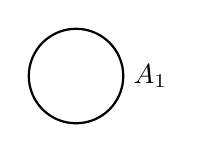
\begin{tikzpicture}

      \draw[thick] (0,0) circle (6mm) node[right=6mm] {$A_1$};

    \end{tikzpicture}
    \caption{Cap end}
    \label{fig:hydraulic-cylinder-2d}
  \end{subfigure}
  \hfill
  \begin{subfigure}[b]{0.3\textwidth}
    \centering
    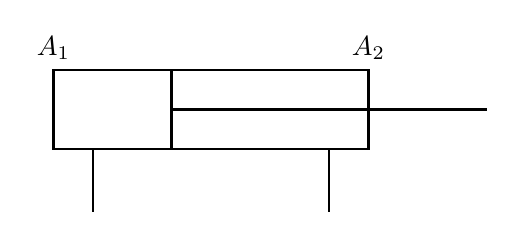
\begin{tikzpicture}

      \draw[thick] (0,0) rectangle (4,1) node[at start, above=10mm] {$A_1$} node[above] {$A_2$};
      \draw[thick] (0.5,0) -- (0.5,-0.8);
      \draw[thick] (3.5,0) -- (3.5,-0.8);
      \draw[very thick] (1.5,0) -- (1.5,1);
      \draw[very thick] (1.5,0.5) -- (5.5,0.5);

    \end{tikzpicture}
    \caption{Hydraulic Cylinder}
    \label{fig:hydraulic-cylinder-2d}
  \end{subfigure}
  \hfill
  \begin{subfigure}[b]{0.3\textwidth}
    \centering
    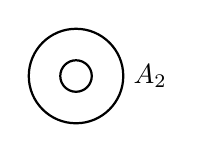
\begin{tikzpicture}

      \draw[thick] (0,0) circle (6mm) node[right=6mm] {$A_2$};;
      \draw[thick] (0,0) circle (2mm);

    \end{tikzpicture}
    \caption{Rod end}
    \label{fig:hydraulic-cylinder-2d}
  \end{subfigure}
  \caption{}
  \label{fig:hydraulic-cylinder}
\end{figure}

\begin{figure}[H]
  \centering
  \begin{subfigure}[b]{0.45\textwidth}
    \centering
    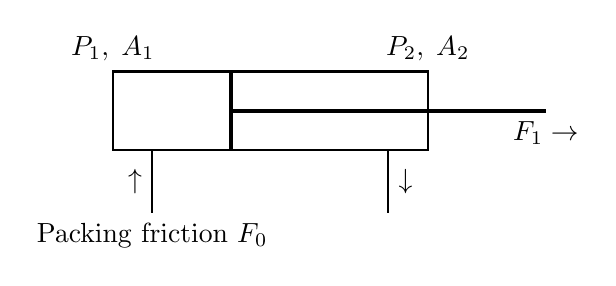
\begin{tikzpicture}

      \draw[thick] (0,0) rectangle (4,1) node[at start, above=10mm] {$P_1,\; A_1$} node[above] {$P_2,\; A_2$};
      \draw[thick] (0.5,0) -- (0.5,-0.8) node[midway, left] {$\uparrow$} node[below] {Packing friction $F_0$};
      \draw[thick] (3.5,0) -- (3.5,-0.8) node[midway, right] {$\downarrow$};
      \draw[very thick] (1.5,0) -- (1.5,1);
      \draw[very thick] (1.5,0.5) -- (5.5,0.5) node[below] {$F_1 \rightarrow$};

    \end{tikzpicture}
    \caption{Hydraulic Cylinder expressed in force with pressure $P_1$/$P_2$, areas $A_1$/$A_2$, and force $F_0$/$F_1$.}
    \label{fig:hydraulic-cylinder-force}
  \end{subfigure}
  \hfill
  \begin{subfigure}[b]{0.45\textwidth}
    \centering
    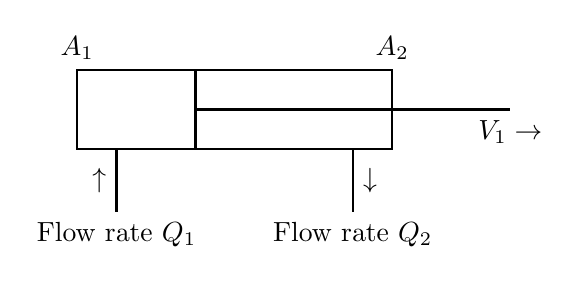
\begin{tikzpicture}

      \draw[thick] (0,0) rectangle (4,1) node[at start, above=10mm] {$A_1$} node[above] {$A_2$};
      \draw[thick] (0.5,0) -- (0.5,-0.8) node[midway, left] {$\uparrow$} node[below] {Flow rate $Q_1$};
      \draw[thick] (3.5,0) -- (3.5,-0.8) node[midway, right] {$\downarrow$} node[below] {Flow rate $Q_2$};
      \draw[very thick] (1.5,0) -- (1.5,1);
      \draw[very thick] (1.5,0.5) -- (5.5,0.5) node[below] {$V_1 \rightarrow$};

    \end{tikzpicture}
    \caption{Hydraulic Cylinder expressed in speed with flow rate $Q_1$/$Q_2$, areas $A_1$/$A_2$, and speed $V_1$.}
    \label{fig:hydraulic-cylinder-speed}
  \end{subfigure}
  \caption{}
  \label{fig:hydraulic-cylinder-force-vs-speed}
\end{figure}





\section{Hydraulic Schematics}

\begin{tikzpicture}
  \pic at (0,0) {pump={Pump 1}};
  \pic at (2,0) {valve={Valve A}};
  \draw[thick] (0.5,0) -- (1.5,0); % Connect pump to valve
\end{tikzpicture}


\begin{tikzpicture}
  \pic (myvalve1) at (0,0) {dcv={control mechanism=lever}};
  \pic (myvalve1) at (4,0) {dcv={control mechanism=pedal}};
  \pic (myvalve1) at (8,0) {dcv={control mechanism=solenoid}};
\end{tikzpicture}


\section{Series and Parallel Hydraulic Circuits}

\section{Hydronic Cylinder}
\section{Check Valves}
\section{Pressure Relief Valves}
\section{Directional Control Valves}

\section{Accumulators}
%\section{Fluid Properties}?
\section{Filters and Conditioning}
\section{Hydraulic Pumps}
\subsection{Gear Pumps}
\subsection{Vane Pumps}
\subsection{Piston Pumps}

\section{Flow Control Valves}
\section{Flow Control Methods}
\subsection{Meter In}
\subsection{Meter Out}
\subsection{Bypass}

\section{Vented and Remote Controlled Pressure Relief Valves}
\section{Sequence Valves}
\section{Pressure Reducing Valves}
\section{Introduction to Electronically Controlled Systems}
\section{Control Relays}



%%% Local Variables:
%%% TeX-master: "../../main"
%%% End:
